% ViT-Tiny / ImageNet-1k validation curve (bf16, 4x 4060 Ti). pgfplots.
% Requires \usepackage{pgfplots} in the preamble (already loaded for the R34 curve).
\begin{center}
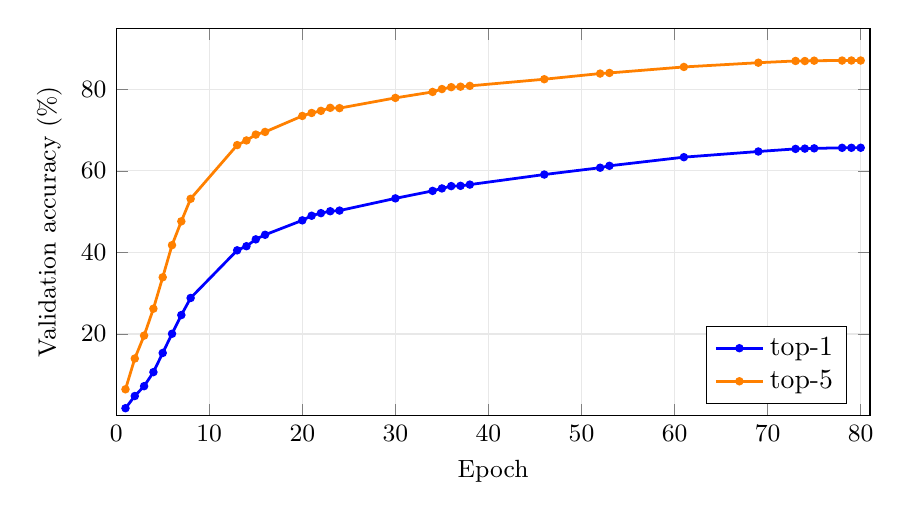
\begin{tikzpicture}
\begin{axis}[
    width=0.92\linewidth, height=6.5cm,
    xlabel={Epoch}, ylabel={Validation accuracy (\%)},
    xmin=0, xmax=81, ymin=0, ymax=95,
    xtick={0,10,20,30,40,50,60,70,80},
    ytick={20,40,60,80},
    legend pos=south east,
    legend cell align={left},
    grid=major, grid style={gray!18},
    tick label style={font=\small},
    label style={font=\small},
    every axis plot/.append style={line width=1pt, mark size=1pt},
]
\addplot[blue, mark=*, mark options={fill=blue}] coordinates {
(1,1.79) (2,4.78) (3,7.20) (4,10.64) (5,15.34) (6,20.05) (7,24.64) (8,28.83) (13,40.52) (14,41.53) (15,43.21) (16,44.33) (20,47.87) (21,49.00) (22,49.64) (23,50.11) (24,50.27) (30,53.26) (34,55.10) (35,55.70) (36,56.27) (37,56.34) (38,56.64) (46,59.11) (52,60.78) (53,61.25) (61,63.37) (69,64.76) (73,65.40) (74,65.47) (75,65.53) (78,65.66) (79,65.67) (80,65.68)
};
\addlegendentry{top-1}
\addplot[orange, mark=*, mark options={fill=orange}] coordinates {
(1,6.43) (2,13.98) (3,19.60) (4,26.20) (5,33.91) (6,41.79) (7,47.63) (8,53.16) (13,66.33) (14,67.47) (15,68.91) (16,69.56) (20,73.48) (21,74.21) (22,74.73) (23,75.47) (24,75.40) (30,77.91) (34,79.37) (35,80.08) (36,80.54) (37,80.66) (38,80.86) (46,82.49) (52,83.88) (53,84.03) (61,85.50) (69,86.54) (73,86.97) (74,86.95) (75,87.04) (78,87.07) (79,87.08) (80,87.08)
};
\addlegendentry{top-5}
\end{axis}
\end{tikzpicture}
\end{center}

\noindent ViT-Tiny / ImageNet-1k validation accuracy per epoch (bf16,
4$\times$ 4060 Ti, sampled). Final: $\mathbf{65.6\%}$ top-1 /
$\mathbf{87.1\%}$ top-5.
